\documentclass[tikz,border=5pt]{standalone}
\usepackage{tikz}
\usetikzlibrary{arrows.meta, positioning}
%\usepackage{times} % Use the times font
\usepackage{palatino} % Uncomment to use the Palatino font
\usepackage{graphicx} % Required for including images
\usepackage{pgfplots}  % For TIKZ plots
\pgfplotsset{compat=1.18}  % Version of the package? 

\begin{document}
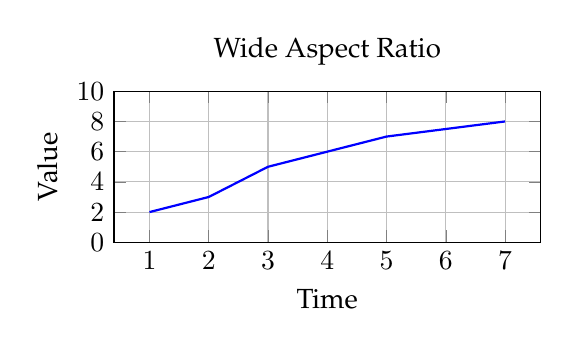
\begin{tikzpicture}
% First plot: wide aspect ratio
\begin{axis}[
    width=7cm,
    height=3.5cm,
    title={Wide Aspect Ratio},
    xlabel=Time,
    ylabel=Value,
    xtick={1,2,3,4,5,6,7},
    ymin=0, ymax=10,
    grid=major
]
\addplot[color=blue, thick] coordinates {(1,2) (2,3) (3,5) (4,6) (5,7) (6,7.5) (7,8)};
\end{axis}
\end{tikzpicture}

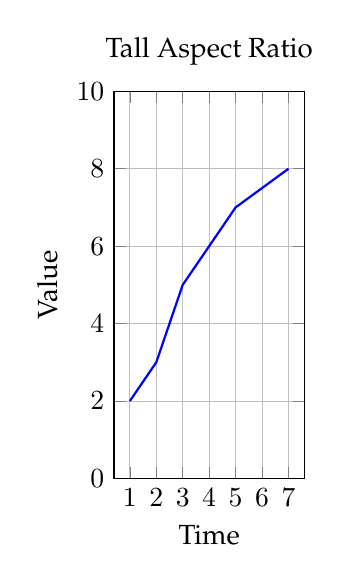
\begin{tikzpicture}

% Second plot: tall aspect ratio
\begin{axis}[
    width=4cm,
    height=6.5cm,
    title={Tall Aspect Ratio},
    xlabel=Time,
    ylabel=Value,
    xtick={1,2,3,4,5,6,7},
    ymin=0, ymax=10,
    grid=major
]
\addplot[color=blue, thick] coordinates {(1,2) (2,3) (3,5) (4,6) (5,7) (6,7.5) (7,8)};
\end{axis}
\end{tikzpicture}

\end{document}